\documentclass[]{article}

\begin{document}
\section{Keuze programmeertaal: Java}
We hebben gekozen voor Java omwille van het grote aanbod van uitgebreide API's. Beide teamleden zijn bekend met de programmeertaal door de cursus object-geori\"{e}nteerd programmeren 2. Ook is de taal cross-platform wat een eis is van het project. Java biedt ook een sterke GUI libary aan nl. Swing.
\section{Algoritme en datastructuren}
\label{Algoritme}
Zoals al eerder vermeld in dit verslag is dient onze applicatie om event-driven programma's te maken. In de volgende sectie halen we kort aan wat het event-driven programming paradigma inhoudt en hoe we dit gaan implementeren. Verder halen we ook aan hoe we onze uitvoer gaan controlleren. Hier verkiezen we concurrent programming. We leggen onze keuze uit met voor en nadelen.
\subsection{Event-driven programming.}
Event-driven programming is een programmeer paradigma waarbij de flow van het programma wordt bepaald door events gecree\"{e}rd door de gebruiker zoals input events of door events veroorzaakt door delen in het programma \cite{eventdrivenwiki}.

\subsubsection{Extended handlers design pattern}
Als design pattern voor onze applicatie basseren we ons op het extended handlers design pattern dat Stephen Ferg uitlegt in zijn paper: Event-Driven Programming: Introduction, Tutorial, History \cite{eventdrivenStephen}.
\begin{figure}[H]
  \centering
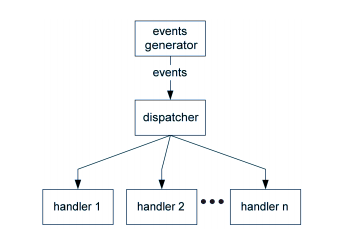
\includegraphics[scale=0.5]{AnalyseADTAlgorithm/extendedHandlerspattern.png}
  \caption{Extended handler.} \label{extendedHandler}
\end{figure}

In Figuur \ref{extendedHandler} stelt de eventgenerator in onze applicatie het generenen van events door gebruikers input en door instanties voor. Door dat events talrijk gegenereerd kunnen worden zal de Dispatcher een queue zijn die een stroom van events opvangt. Hij zal ervoor zorgen dat het event door de juiste handelers wordt afgewerkt.\\\\
Doordat in onze applicatie events worden doorgegeven aan specifieke andere instanties van Klassen zoals beschreven in de Sectie \ref{Events}. Zal de dispatcher ervoor moeten zorgen dat de juiste handlers van de juiste instanties worden aangeroepen.

\subsection{Concurrent computing }
Concurrent computing \cite{concurrent} is een vorm van computing waarbij een deel berekeningen worden uitgevoerd zodat het lijkt alsof ze gelijktijdig worden uitgevoerd. We hebben ervoor gekozen om niet multi-threaded te werken om de complexiteit van het project zo laag mogelijk te houden.\\\\ Daarom is concurrent computing de oplossing voor onze applicatie. In tegenstelling tot parallel computing is dit wel mogelijk op een thread. Gelijktijdige processen zoals twee events die samen worden opgeroepen lijken hierdoor ook gelijk te worden afgehandeld. In tegenstelling tot het sequentiel uitvoeren van de twee events.\\\\
Bij concurrent computing worden processen in executie stappen opgedeeld. Er wordt gebruik gemaakt van timeslices waarin van elk proces een deel executie stappen worden uitgevoerd, wij noemen dit een primitieve stap. Na dat bepaald aantal of tijd wordt het proces gepauzeerd en verder gegaan met het volgende. Dit wordt herhaald zolang een proces niet volledig is afgerond.
\subsubsection{Verschil met parallel computing}
Parallel computing is gelijkaardig aan concurrent computing, echter gebeurt het werk op verschillende cores. Bij concurrent computing zal de uitvoering van twee identieke events die gelijktijdig worden aangeroepen niet gelijktijdig eindigen omdat de uitvoering steeds wisselt tussen de twee events. 

\subsubsection{Probleem met concurrent computing}
Een eerste probleem is racing conditions. Hierbij proberen twee processen hetzelfde algortime uit te voeren waarbij een bepaalde sequentie van uitvoering belangrijk is. Het volgende voorbeeld gevonden op \cite{concurrent} toont een functie waarbij een private member variabele balance wordt geaccessed en verandered. Stel dat er twee processen runnen die respectievelijk withdraw(200) en withdraw(300) oproepen en dat balance 250 bedraagt. Bij beide processen zal de conditie 250 $>$ withdrawal, slagen, want balance is nog niet aangepast. Echter zal hierna balance aangepast worden en uiteindelijk -250 bedragen. Dit is een verkeerde uitvoering.
\lstset{language=Java}
\begin{lstlisting}
public class Main {
	public boolean withdraw(int withdrawal) {
    	if (balance >= withdrawal) {
        	balance -= withdrawal;
        	return true;
    	}	 
    	return false;
	}
}
\end{lstlisting}
Onze oplossing hiervoor is een lock op een private member variabele toelaten. Deze zorgt dan dat enkel dat proces aan die variabele kan voor zowel te lezen als te schrijving.\\\\
Hierbij komt een ander probleem tevoorschijn, nl. een deadlock \cite{deadlock}. Om dit probleem op te lossen stellen we dat slechts \'{e}\'{e}n proces gelijktijdig locks kan aanbrengen.

\subsection{Drawing}
\paragraph{Blokken}worden getekend door middel van rechthoeken. Deze kunnen genest worden in elkaar.
\paragraph{Het WireFrame}is de collectie van Instances en Wires. Een Instance wordt getekend als een blok waarop enkele punten getekend zijn die de inkomende en uitgaande Events voorstellen. De Wires worden getekend als lijnen. Deze lijn kan bestaan uit meerdere punten en wordt getekend door de gebruiker. Deze lijn zal dus niet automatisch gegenereerd worden.

\subsection{Model en Controller}
Elke visuele component is verbonden met een model (zie Sectie \ref{ModelBlock}). Dit model bevat info die nodig is om aan type checking te doen in de GUI. Ook worden de blokken die genest zitten in deze blok bijgehouden in het model. De wireFrame zal ook voorgesteld worden als een Model. De controller die behoort tot een model zal nagaan of een blok genest kan worden in een bestaande blok door informatie op te vragen aan het model van de bestaande block. Er wordt ook doorgegeven wanneer er iets genest wordt.

\subsection{Runtime}
\label{Runtime}
Op het hoogste niveau is een Runtime (zie Sectie \ref{runtimeClass}) aanwezig. De IDE gebruikt een Abstracte klasse Runtime zodanig dat de gebruikte programmeertaal niet direct vasthangt aan de IDE. Er is een klasse aanwezig die de Runtime voor de ge\"{i}mplementeerde programmeertaal implementeerd. De abstracte Runtime bevat alle modellen van de blocks alsook het wireFrame model, de ge\"{i}mplementeerde Runtime bevat de nodige data voor de executie van de code zoals een Compiler en een Virtual Machine (zie Sectie \ref{VM}). De Runtime zorgt voor de vlotte uitvoering van alle code. Er is een functie aanwezig die continue de Virtual Machine aanroept zolang er niet gestopt moet worden. Door een aparte thread aan te maken zal hij deze functie parallel kunnen runnen met de GUI. Verdere executie is uitgelegd in Sectie \ref{VM}.

\subsection{Compileren}
\label{Compileer}
Elke visuele view van een blok heeft een model zoals uitgelegd. Deze blok wordt bij het compileren meegegeven aan een Compiler Klasse door de Runtime. Deze klasse is een information expert met betrekking tot compileren. De IDE gebruikt een Interface Compiler zodanig dat de gebruikte programmeertaal niet direct vasthangt aan de IDE. Hij heeft verschillende functies die elk een ander type BlockModel (\ref{ModelBlock}) compileren. Omdat het wireFrame ook voorgesteld wordt als een model kan het wireFrame simpel gecompileerd worden omwille van deze functies. Elk model weet welke blokken genest zijn zullen alle geneste blokken ook worden gecompileerd. Het design van de Compiler is het visitor design pattern. Het algoritme voor het compilen van een blok wordt gescheiden van de datastructuur van de blok.  

\subsection{Virtual Machine}
\label{VM}
Onze virtual machine bevat een lijst van alle processen die momenteel moet uitgevoerd worden. Incrementeel zal er telkens \'{e}\'{e}n  primitieve stap uitgevoerd worden van elk proces. Als er een proces uitgevoerd moet worden, zal dit toegevoegd worden aan het einde van de lijst. Als een bepaald proces klaar is, wordt dit verwijderd uit de lijst. \\\\
Als een Event verstuurd wordt zal de Virtual Machine dit Event doorgeven aan een Event Dispatcher. Dit is een Klasse die de taak voor het verzenden van Events op zich neemt. De Event Dispatcher kent alle verbindingen tussen de Instanties, en hiermee kunnen nieuwe processen aangemaakt worden zodat de Virtual Machine deze kan gebruiken. 
\subsubsection{Een proces}
Een proces (zie Sectie \ref{procesklass}) is een gesimuleerde thread. Deze beheert nodige data zoals een variable-stack en code. Een proces wordt uitgevoerd door de VM. Een proces kan gerunned worden en deze zal dan \'{e}\'{e}n primitieve stap \ref{primitive}uitvoeren.
\subsubsection{Stoppen van uitvoering}
Voor het stoppen van de uitvoer zal er een event worden verzonden naar de Runtime bij het opvangen van dit event zal de uitvoering worden gestopt.

\subsection{Voorbeeld implementatie}
\label{voorbeeldvm}
Er bestaat een Klasse die een input event: event1 accepteerd. Dit event wordt afgehandeld door handler1 van de Klasse. De gebruiker heeft deze handler ge\"{i}mplementeerd in blokken op de volgende manier:
\lstset{language=Java}
\begin{lstlisting}
Event event1{
	members:
		- member1(number, value)
}
class Class1 {

	handler( event1) {
    		makeVar(number, x)
    		set(X, acces(event1, member1)
    		functieCall(functie1, parameters: x, return:x)
	}
	
	functie(functie1, parameters: z){
		while(z < 10){
		set(z, z + 1)
		}
		return z;
			
	}
	
	
}
\end{lstlisting}
Instantie instance1 is een instantie van Class1 waarnaar een instantie van event1 wordt verzonden. De eventDispatcher zal dus een proces aanmaken met instantie1 en op de Code stack de handler pushen.\\
Het uitvoeren van het proces zal in de volgende primitieve stappen gebeuren:\\\\
\textbf{Stap 1:} De handler zal zijn execute functie uivoeren. Deze zal een nieuw FunctieFrame aanmaken. Ook zal de eventInstance die mee werd gegeven bij het aanmaken van het proces op de stackframe geduwd. De blok van de handler op de Stack wordt vervangen door de inhoud.\\
\textbf{Stap 2:} De execute van makeVar zal een nieuwe variable van het type number maken op het huidige FunctieFrame.\\
\textbf{Stap 3:} De execute van Set zal de het Event in de huidige Stackframe zoeken en hieruit de juiste member halen nl. member1. De waarde hiervan wordt in x geplaatst. We gaan er van uit dat member1 $=$ 8.\\
\textbf{Stap 4:} De execute van FunctieCall doet de volgende stappen. Ophalen van de de parameter waarde die in de call staan. Deze slaat gij op in volgorde van de oproep. Hierna haalt hij het functieblok met de juiste functie naam op. Hiervan haalt hij de parameter namen op. Hij cree\"{}ert een nieuw FunctieFrame en daarop pushed hij de parameternamen met de juiste eerder opgehaalde waarde. Hier is dit dus z met de waarde 8. Dit gebeurt achter de schermen met makeVar- en set-blokken. Hierna worden er eerst nog set-blokken voor de return waardes op de stack gepushed. Nu wordt de execute van de functie aangeroepen. Deze zal al zijn blokken op de stack pushen zonder nieuw frame te cree\"{e}ren.\\
\textbf{Stap 5:} De bovenste blok is nu de While blok. De execute van deze blok zal zijn conditie controleren nl $z < 10$ deze evalueert naar true aangezien x $=$ 8. Hierdoor zal de body van de While-blok op de code stack worden gepushed. Maar eerst wordt de While-blok er zelf ook nog op gepusht.\\
\textbf{Stap 6:} De waarde van X wordt in de set-blok verhoogt met 1.\\
\textbf{Stap 7:} herhaling stap 5.\\
\textbf{Stap 8:} herhaling stap 6.\\
\textbf{Stap 9:} De conditie van de While-blok evalueert nu naar false. Hierdoor worden er geen blokken op de code stack gepusht.\\
\textbf{Stap 10:} De return blok zoekt in de huidige FunctieFrame de waarde van z op en plaats deze in de returnVariables.\\
\textbf{Stap 11:} Aangezien de functie is afgelopen mag het FunctieFrame van de stack worden gepopt.\\
\textbf{Stap 12:} De set-blok zal nu x in het huidige FunctieFrame veranderen naar de return waarde\\
\textbf{Stap 13:} Het proces bevat geen blokken meer dus zal een ProcesFinishedException gooien naar de VM deze zal het proces verwijderen uit de queue.
 
\begin{figure}[H]
\centering
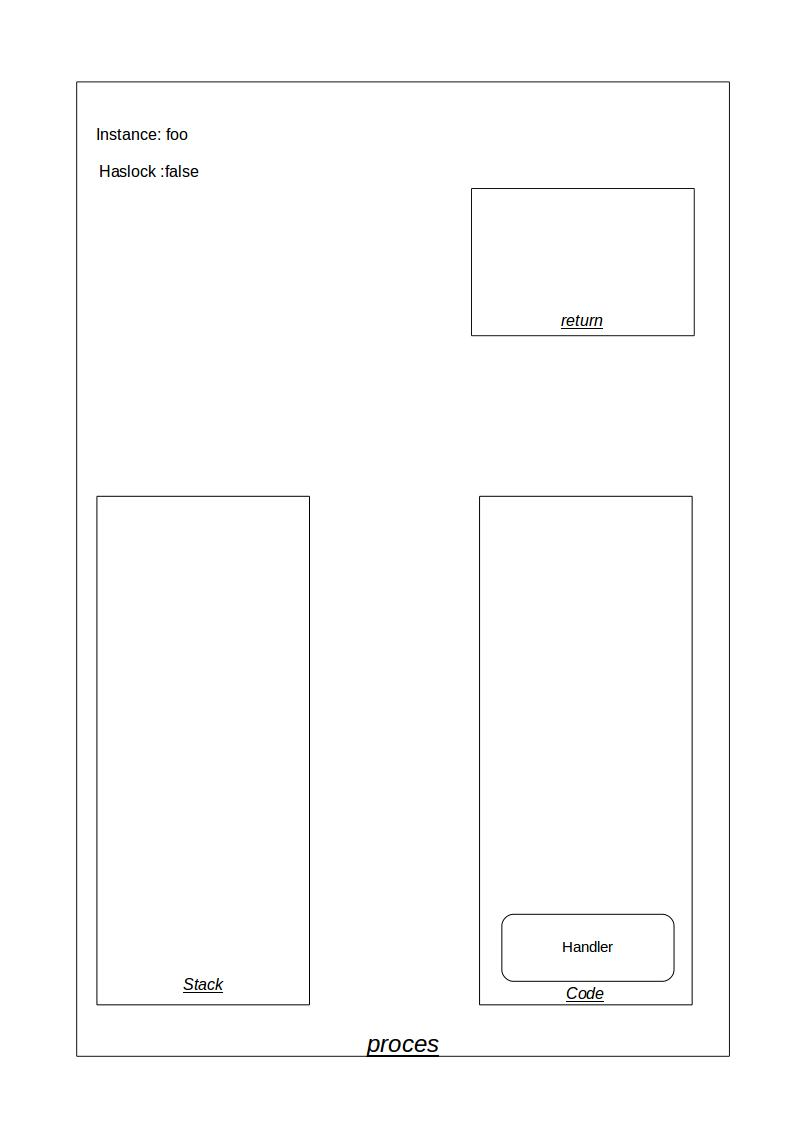
\includegraphics[scale=0.4]{AnalyseADTAlgorithm/processtappen/stap1.jpg}
\caption{Stap 1}
\end{figure}

\begin{figure}[H]
\centering
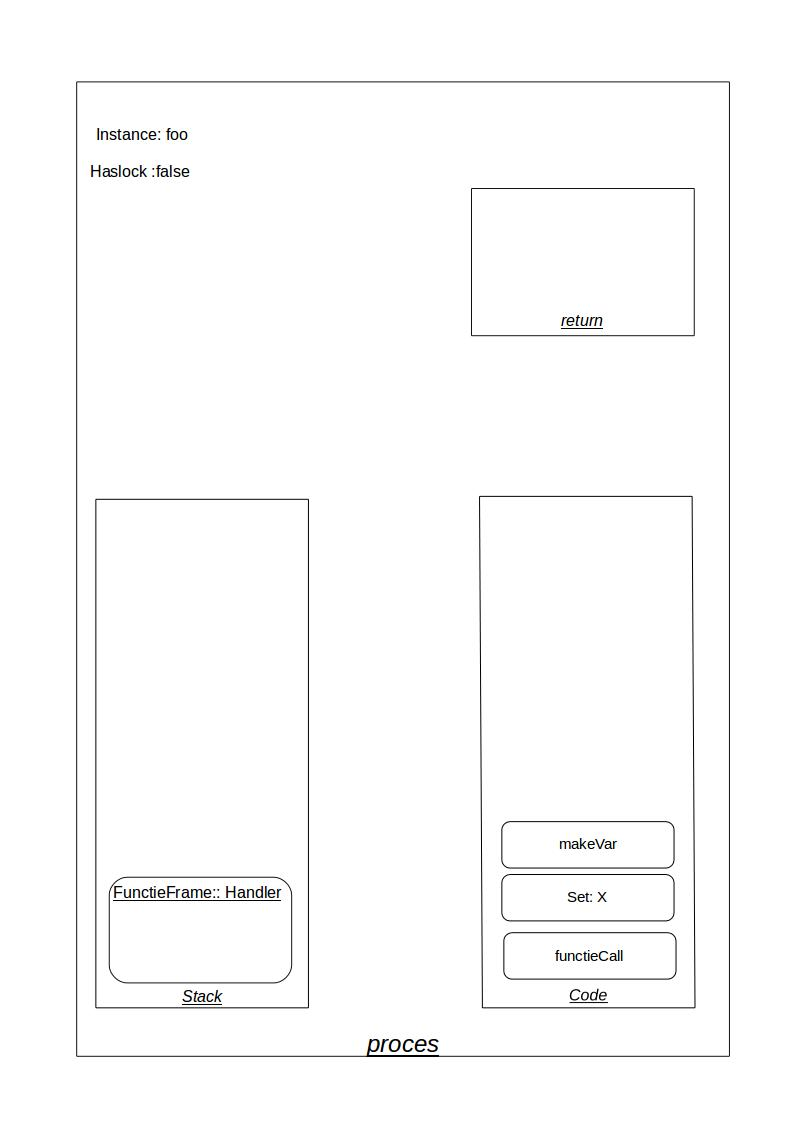
\includegraphics[scale=0.4]{AnalyseADTAlgorithm/processtappen/stap2.jpg}
\caption{Stap 2}
\end{figure}

\begin{figure}[H]
\centering
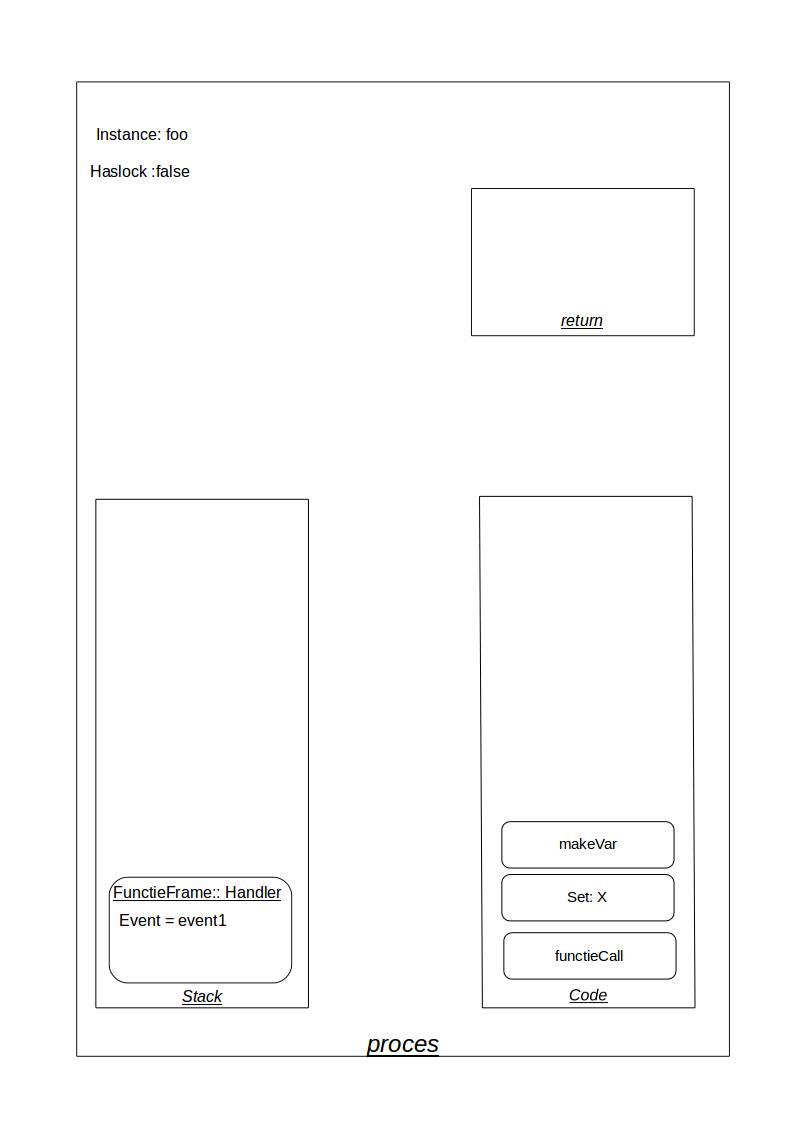
\includegraphics[scale=0.4]{AnalyseADTAlgorithm/processtappen/stap3.jpg}
\caption{Stap 3}
\end{figure}
\begin{figure}[H]
\centering
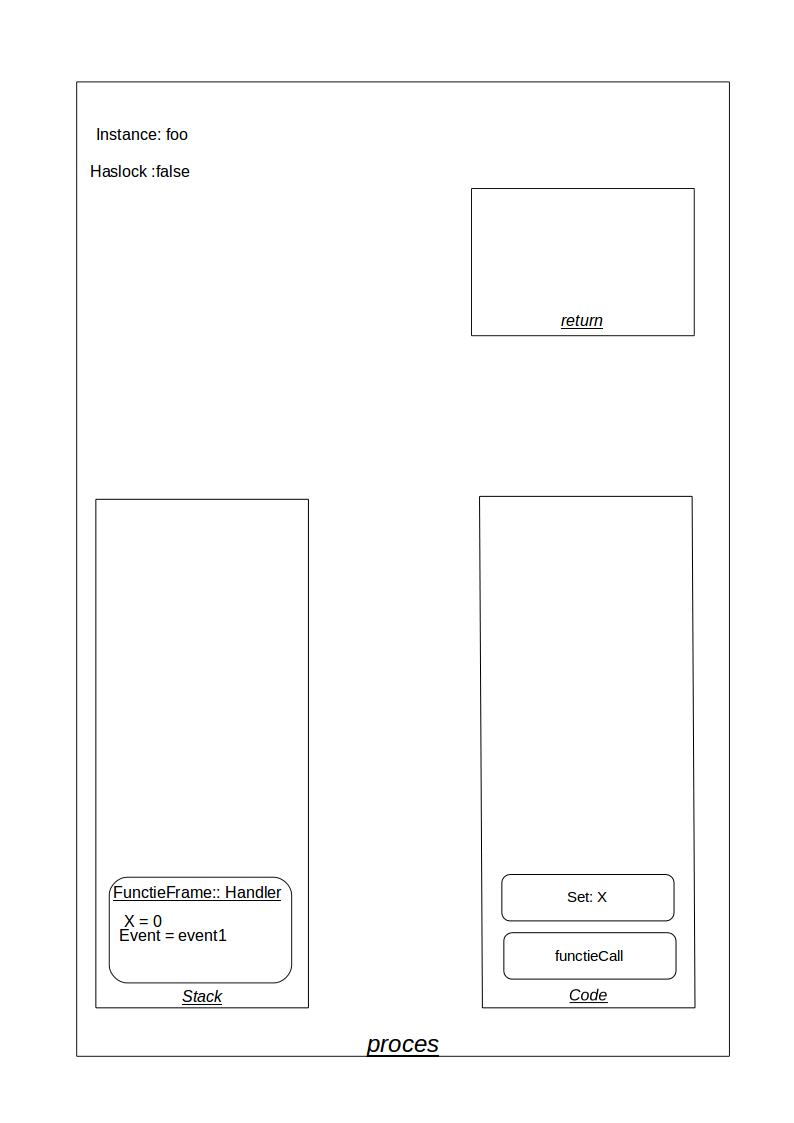
\includegraphics[scale=0.4]{AnalyseADTAlgorithm/processtappen/stap4.jpg}
\caption{Stap 4}
\end{figure}
\begin{figure}[H]
\centering
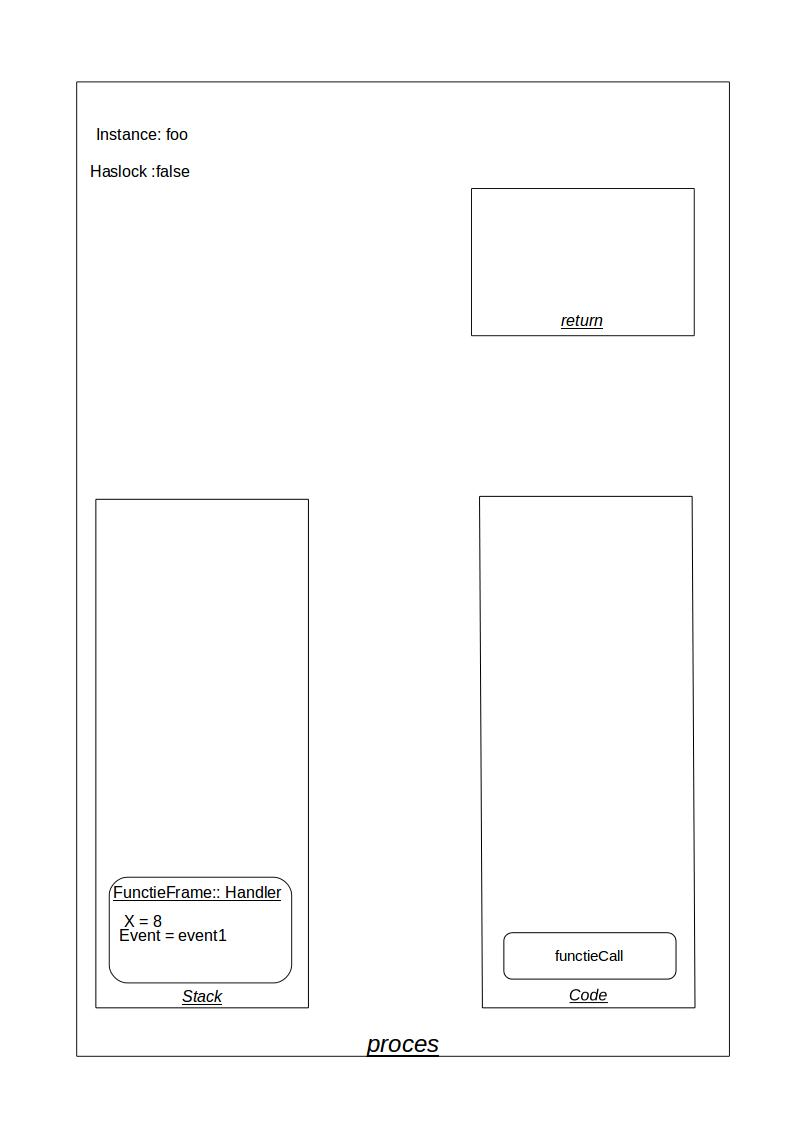
\includegraphics[scale=0.4]{AnalyseADTAlgorithm/processtappen/stap5.jpg}
\caption{Stap 5}
\end{figure}

\begin{figure}[H]
\centering
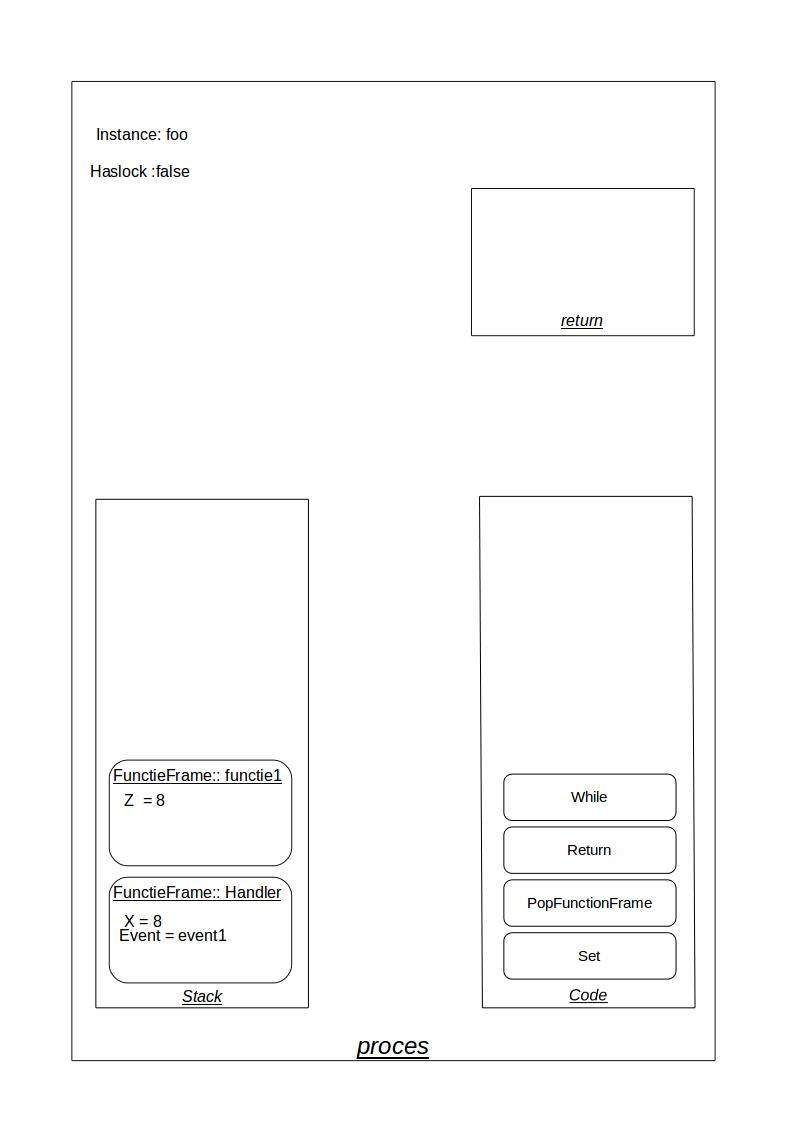
\includegraphics[scale=0.4]{AnalyseADTAlgorithm/processtappen/stap6.jpg}
\caption{Stap 6}
\end{figure}

\begin{figure}[H]
\centering
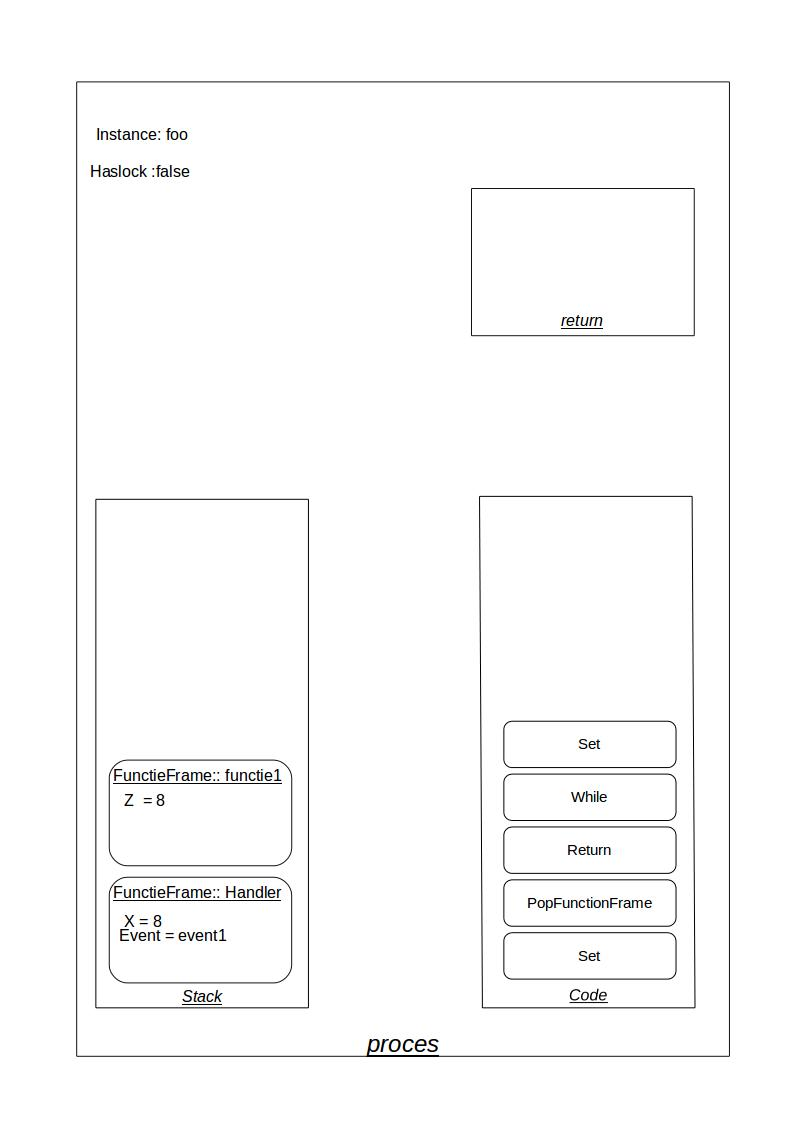
\includegraphics[scale=0.4]{AnalyseADTAlgorithm/processtappen/stap7.jpg}
\caption{Stap 9}
\end{figure}

\begin{figure}[H]
\centering
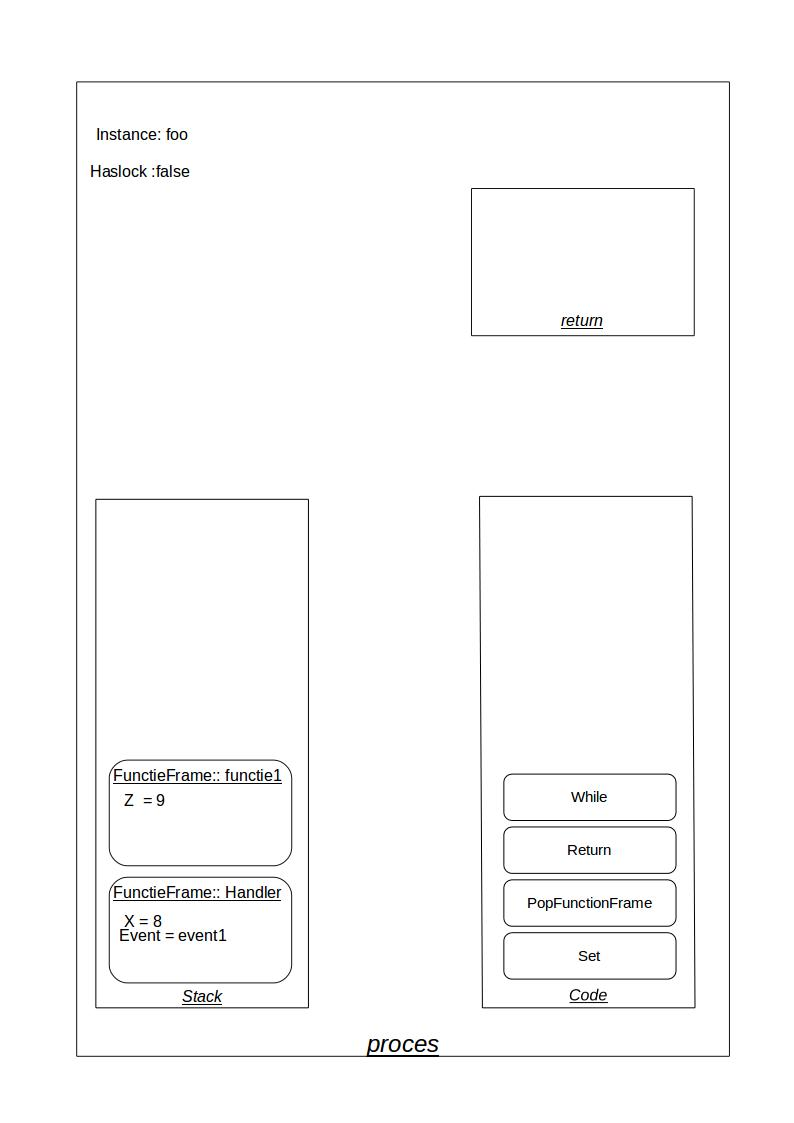
\includegraphics[scale=0.4]{AnalyseADTAlgorithm/processtappen/stap8.jpg}
\caption{Stap 10}
\end{figure}

\begin{figure}[H]
\centering
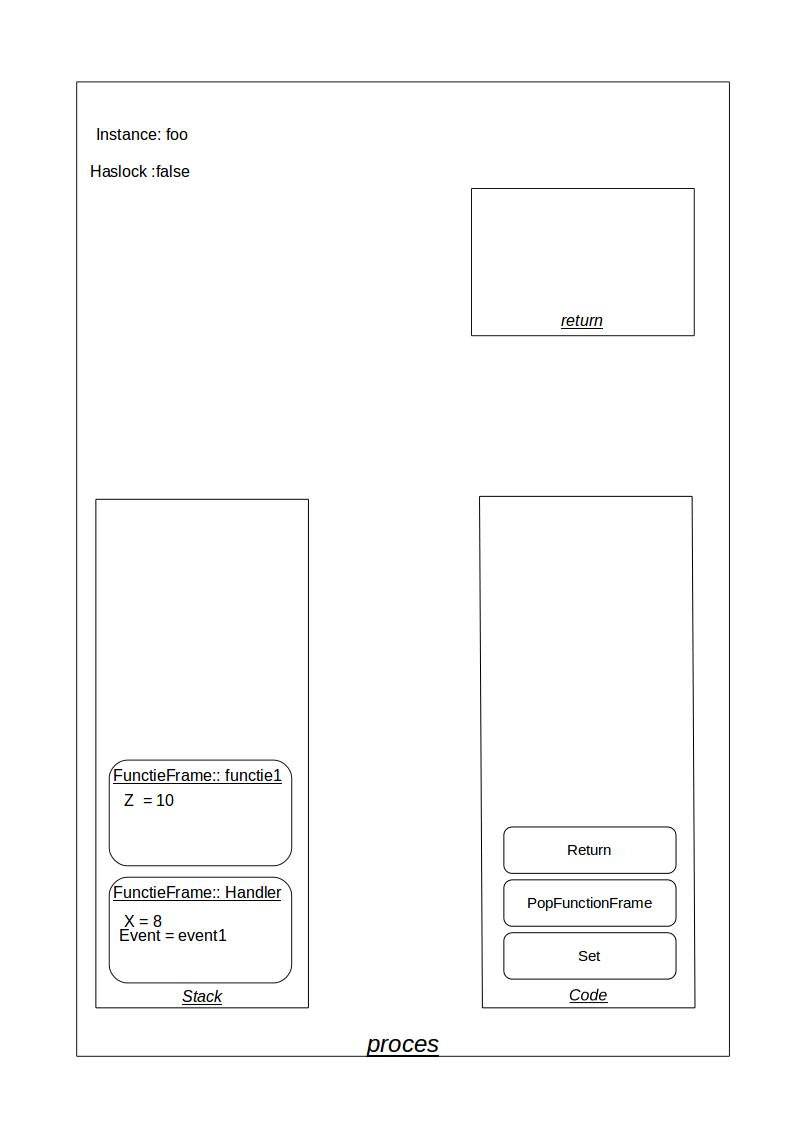
\includegraphics[scale=0.4]{AnalyseADTAlgorithm/processtappen/stap9.jpg}
\caption{Stap 11}
\end{figure}
\begin{figure}[H]
\centering
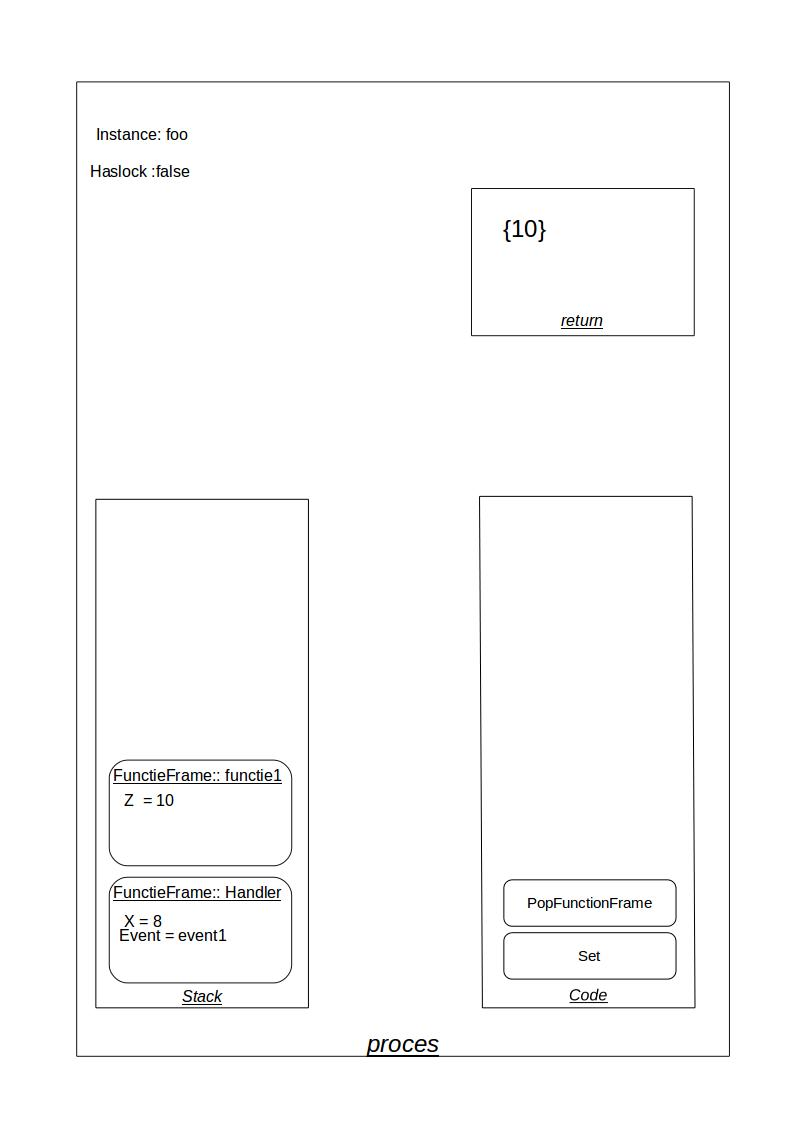
\includegraphics[scale=0.4]{AnalyseADTAlgorithm/processtappen/stap10.jpg}
\caption{Stap 12}
\end{figure}
\begin{figure}[H]
\centering
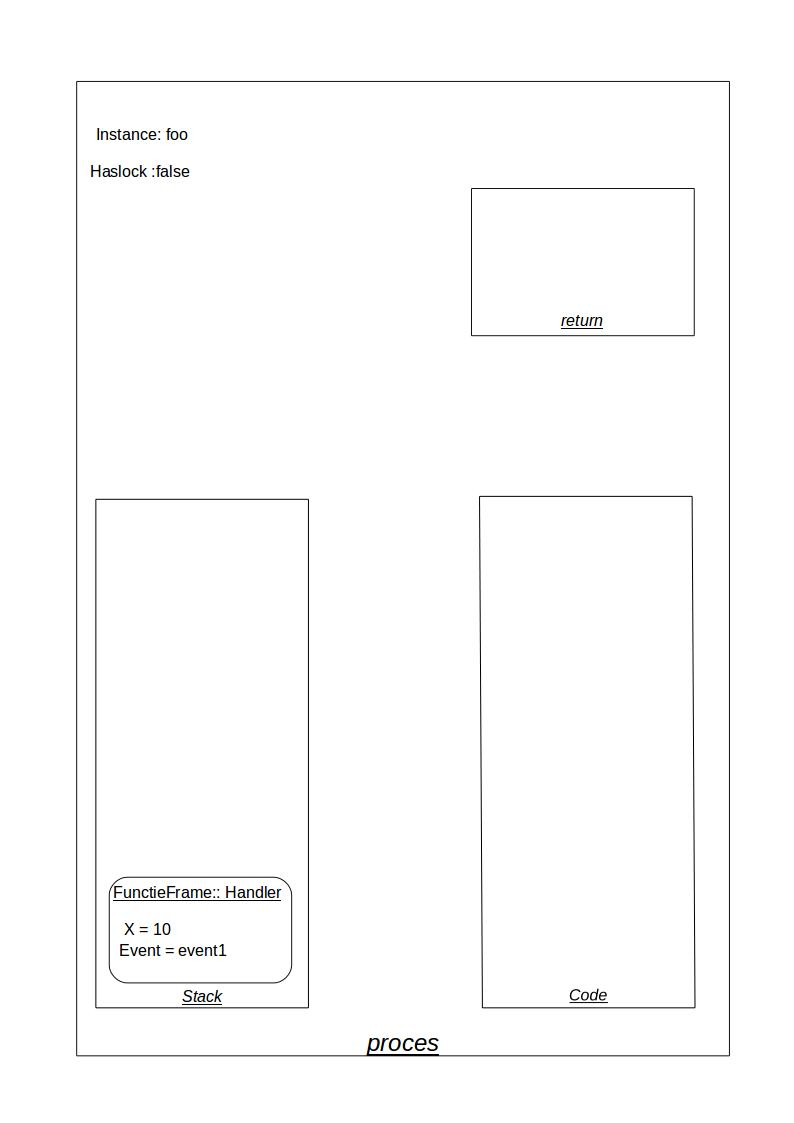
\includegraphics[scale=0.4]{AnalyseADTAlgorithm/processtappen/stap11.jpg}
\caption{Stap 13}
\end{figure}

\subsection{Lambda expressions}
\label{lambda}
Sinds 1.8 biedt java de mogelijk aan om lambda expressions \cite{lambda} te gebruiken, we gaan hier dan ook gebruik van maken. Onze operator blok is hier geschikt voor. Via lambda expressions kan men anonieme interface methodes aanmaken. Hieronder volgt een voorbeeld waarin duidelijk volgt hoe wij het zouden gebruiken. 
\lstset{language=Java}
\begin{lstlisting}
public class Calculator {
  
    interface IntegerMath {
        int operation(int a, int b);   
    }
  
    public int operateBinary(int a, int b, IntegerMath op) {
        return op.operation(a, b);
    }
 
    public static void main(String... args) {
    
        Calculator myApp = new Calculator();
        IntegerMath addition = (a, b) -> a + b;
        IntegerMath subtraction = (a, b) -> a - b;
        System.out.println("40 + 2 = " +
            myApp.operateBinary(40, 2, addition));
        System.out.println("20 - 10 = " +
            myApp.operateBinary(20, 10, subtraction));    
    }
}
\end{lstlisting}
In de operator block zal een statische hashmap bijgehouden worden. Deze word slechts \'{e}\'{e}n keer ge\"{i}nitialiseerd. In deze hashmap worden strings gemapt op lambda functies. De string $+$ mapt op een lambda functie enz. Deze lambda functie wordt hieronder beschreven:
\begin{lstlisting}
    interface OperatorMath {
        Variable operation(Variable a, Variable b);   
    }
  
    OperatorMath addition = (a, b) -> a.addVar(b);
    OperatorMath subtraction = (a, b) -> a.subVar(b);
\end{lstlisting}
\section{Code structuur}
Alle code zal opgedeeld worden in verschillende modules. Deze modules defini\"{e}ren hoe er met andere modules gecommuniceerd word. Hierdoor word het gemakkelijk om modules intern van werking te veranderen zonder dat er iets moet veranderen aan andere modules. Een module is een cluster van klassen die instaan voor elk instaan voor een doel dat beschouwd wordt door de module.

\subsection{Exceptions Module}
\label{ExceptionsModule}
Deze module heeft enkel als verantwoordelijkheid om alle excepties te groeperen.

\subsection{Variables Module}
\label{VariablesModule}
Deze module bevat alle klassen die te maken hebben met de data types die gebruikt worden.

\subsection{Blocks Module}
\label{BlocksModule}
Deze module implementeerd alle executie bloks die aanwezig zijn in de IDE.

\subsection{Collections Module}
\label{CollectionsModule}
Deze module bevat klasses die higher level zijn dan blocks. Het zijn collecties van Events, Classes, Instances.

\subsection{Core module}
\label{CoreModule}
Deze module staat in voor het uitvoeren van de code. De output van de compile module \ref{compile} zal door de VM module uitgevoert worden. Deze module kan werken in een release mode waarbij code normaal uitgevoert word, of in een debug modus waarbij er stap voor stap doorgeen het programma gelopen kan worden. 

\subsection{Model module}
\label{ModelModule}
Deze module is de representatie van alle code die gemaakt kan worden in de visuele IDE. Deze module zal ook instaan voor het nakijken van de code op syntax fouten (zie Sectie \ref{ModelBlock}). Deze module heeft verschillende klassen om events, Klassen, instances, variabelen en primitieve code blokken voor te stellen. 

\subsection{Runtime module}
\label{RuntimeModule}
\label{compile}
Deze module zal instaan voor het compilen en runnen van de code. De module zal een bepaalde hoeveelheid ruwe code van Klassen, Instances en Events omvormen naar uitvoerbare code. Deze module bevat ook een klasse die de runtime regelt van de programmeertaal van de IDE.

\subsection{File module}
Deze module behandeld het laden en saven van de IDE data. Deze data omvat de XML data. Er wordt ook gezorgd voor het multilanguage maken van de applicatie (zie Sectie \ref{Multilanguage}).

\subsection{GUI}
De GUI wordt momenteel bekeken als \'{e}\'{e}n grote module maar zal nog opgedeeld worden in kleinere modules zoals een menu module, etc. 



\end{document}